\section*{Suchen in Texten}
\subsection*{Naive Textsuche}

$\mathcal{O}(n*m)$

\textbf{Anzahl Vergleiche:} Textlänge - Musterlänge + 1 (+ Treffer)

\subsection*{Boyer-Moore}

\begin{enumerate}
	\item Suche jeweils das hinterste Zeichen im Text, welches nicht mit dem Muster übereinstimmt
	\item Falls es kein solches gibt (j $<$ 0), wurde das Muster gefunden
	\item Ansonsten (j $\geq$ 0) wird die Position von i anhand des Shift-Arrays verschoben
\end{enumerate}

\subsection*{Vorkommens-Heuristik}

\begin{itemize}
	\item Für alle Zeichen, die im Muster nicht enthalten sind -> Länge des Musters
	\item Zeichen nur an letzter Position im Muster -> Länge des Musters
	\item Sonst Muster-Länge - 1 - lastIndex(Muster, Zeichen)
\end{itemize}

\subsubsection*{Asymptotische Komplexität}
n = Text-Länge, m = Muster-Länge

\textbf{Worst-Case:} $\mathcal{O}(n*m)$

\textbf{Erwarteter Average-Case:} $\mathcal{O}(n/m)$

\textbf{Best-Case:} $\mathcal{O}(m)$ (Muster an erster Stelle)

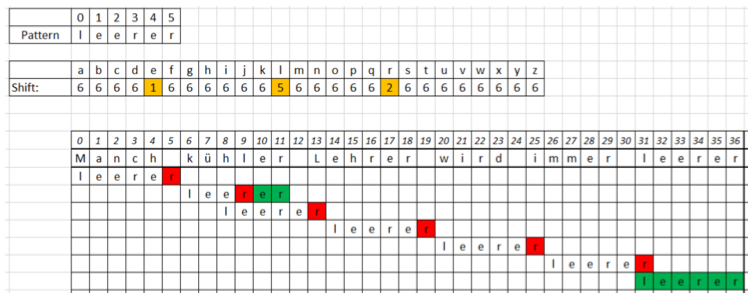
\includegraphics[width=\linewidth]{images/boyermoore}

\begin{minted}[breaklines]{java}
    public int firstMatch(String text, String pattern) {

        int[] shift = allShifts(pattern);

        int l = pattern.length(), i = 0, j = l - 1; // Warum?
        while (i + l <= text.length() && j >= 0) {

            j = l - 1; // Warum?

            while (j >= 0 && pattern.charAt(j) == text.charAt(i + j)) {
                  j--;
            }

            if (j >= 0) {
                i = i + shift[text.charAt(i + l - 1)];
            }
        }
        return (i + l <= text.length()) ? i : -1;
    }
\end{minted}